
\documentclass[11pt,a4paper]{article}

% ---------- Packages ----------
\usepackage[margin=1in]{geometry}
\usepackage{graphicx}
\usepackage{amsmath, amssymb, amsthm}
\usepackage{booktabs}
\usepackage{array}
\usepackage{enumitem}
\usepackage[hidelinks]{hyperref}
\usepackage{titlesec}

% Optional: tighter run-in paragraph/subparagraph spacing
\titlespacing*{\paragraph}{0pt}{1.25ex plus .5ex}{1em}
\titlespacing*{\subparagraph}{0pt}{1.0ex plus .5ex}{1em}

% ---------- Macros ----------
% Common Hamiltonian notation
\newcommand{\Hising}{H_{\mathrm{Ising}}}
\newcommand{\Htf}{H_{\mathrm{TF}}}
\newcommand{\Htot}{H=\Hising+\Htf}
\renewcommand{\footnoterule}{}

% A small helper for nice math in tables
\newcommand{\NNZ}{\#\text{non-zero components}}

% Table column types
\newcolumntype{L}[1]{>{\raggedright\arraybackslash}p{#1}}
\newcolumntype{C}[1]{>{\centering\arraybackslash}p{#1}}

% ---------- Header ----------
\title{Scars of the Transverse Field Ising Model on Discrete Geometries (Polyhedra)}
\author{}
\date{\today}

\begin{document}
\maketitle

% ============================================================
% OVERALL PARAGRAPH (global statement for the whole note)
% ============================================================
\section*{Introduction}
We are studying scars of the simple Ising model on discrete geometries (polyhedra). Here, \emph{scars} are identified as special, sparser eigenstates of the Hamiltonian which are simultaneously eigenstates of the Ising term and of the transverse-field (TF) term separately; in addition, each such state is annihilated by exactly one of the two terms. In all of the following examples, the Hamiltonian is

\begin{equation}
\Htot, \quad \Hising = J \sum_{\langle i,j\rangle} \sigma_i^x \sigma_j^x, \quad  \Htf = - h \sum_i \sigma_i^z
\end{equation}

where $J=1, h=3$ (antiferromagnetic, non critical).

\section*{Platonic Solids}
% ============================================================
% REPEAT THE BLOCK BELOW FOR EACH POLYHEDRON
% ============================================================

% -------------------- Polyhedron Block: START --------------------
\subsection*{Tetrahedron}

\subsubsection*{Overview and data}
\begin{center}
  % Put your graphic at the very beginning of the subparagraph
  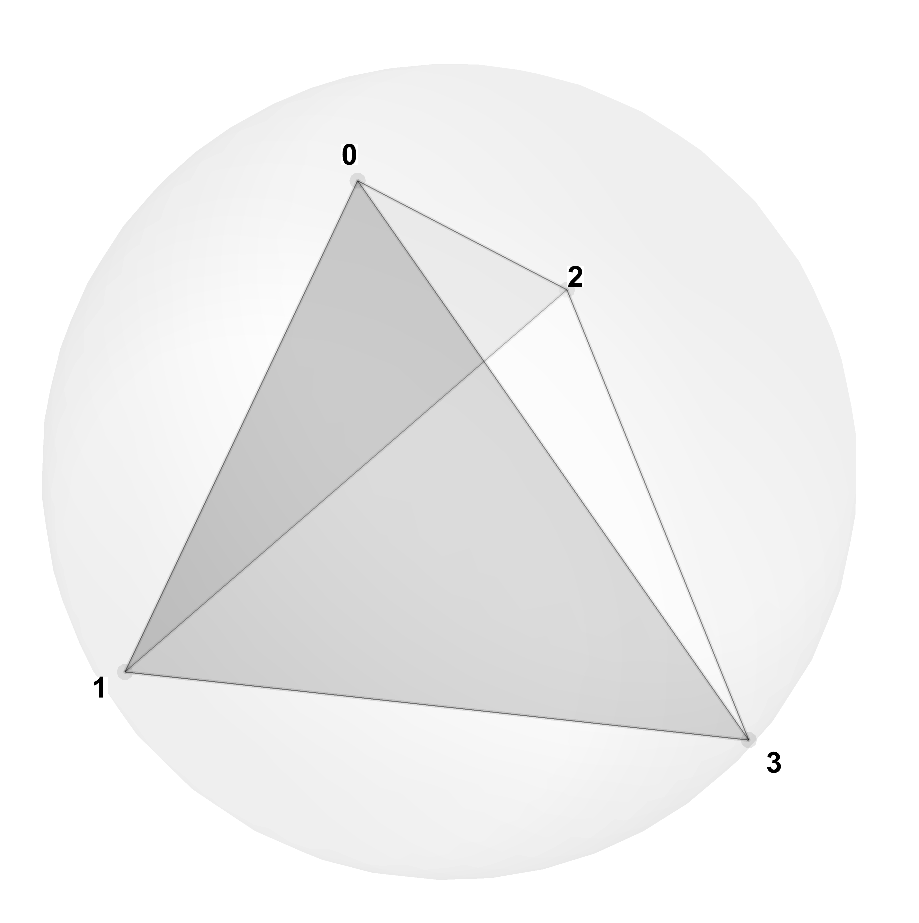
\includegraphics[width=.6\linewidth]{tetrahedron}
\end{center}

\begin{itemize}[leftmargin=1.5em]
  \item \textbf{Duality / paired solid:} self-dual, tetrahedron
  \item \textbf{Vertices (V), Faces (F), Edges (E):} $V = 4$,\; $F = 3$ (equilateral triangles),\; $E = 6$
  \item \textbf{Point group:} $T_d$
  \item \textbf{Hilbert space:} \(
        \dim\mathcal{H} = 2^{4} = 16\ \text{(spin-$\tfrac12$ on each vertex)}
        \)
  \item \textbf{Eigenvalue range:} $[-12.37, 12.71]$
\end{itemize}

\subsubsection*{Scar structure: sets and multiplets}

\begin{itemize}[leftmargin=1.5em]
  \item \textbf{Number of scar sets:} 1
  \end{itemize}
  \hspace{6mm}For each scar set $S_k$:\\

\begin{center}
\begin{tabular}{L{3.5cm} C{2.2cm} C{2.2cm} C{2.2cm} C{3.0cm} C{3.2cm}}
\toprule
\textbf{Multiplet label} & \textbf{Energy $E$} & \textbf{Degeneracy} & \textbf{Annihilated by} & \textbf{Non-zero components (vs.\ $2^{4} = 16$)} \\
\midrule
$S_1$ & -2 & 2 & $\Htf$ & 4,6 \\
\bottomrule
\end{tabular}
\end{center}

\subsubsection*{Local properties (RDMs)}

\begin{itemize}[leftmargin=1.5em]
  \item \textbf{Local RDM definition:} $\rho_A=\mathrm{Tr}_{\bar A}(|\psi\rangle\langle\psi|)$ on compact subsets of $n=1$ sites, with $n < V/2, (V = 4)$
  \item \textbf{Compactness criterion:} NA, the single point ${0}$ was chosen
  \item \textbf{Diagnostics:} 1-site RDMs for both scars have full rank (system size $V=4$ is too small)
\end{itemize}

% -------------------- Polyhedron Block: END --------------------

% -------------------- Polyhedron Block: START --------------------
\subsection*{Octahedron}

\subsubsection*{Overview and data}
\begin{center}
  % Put your graphic at the very beginning of the subparagraph
  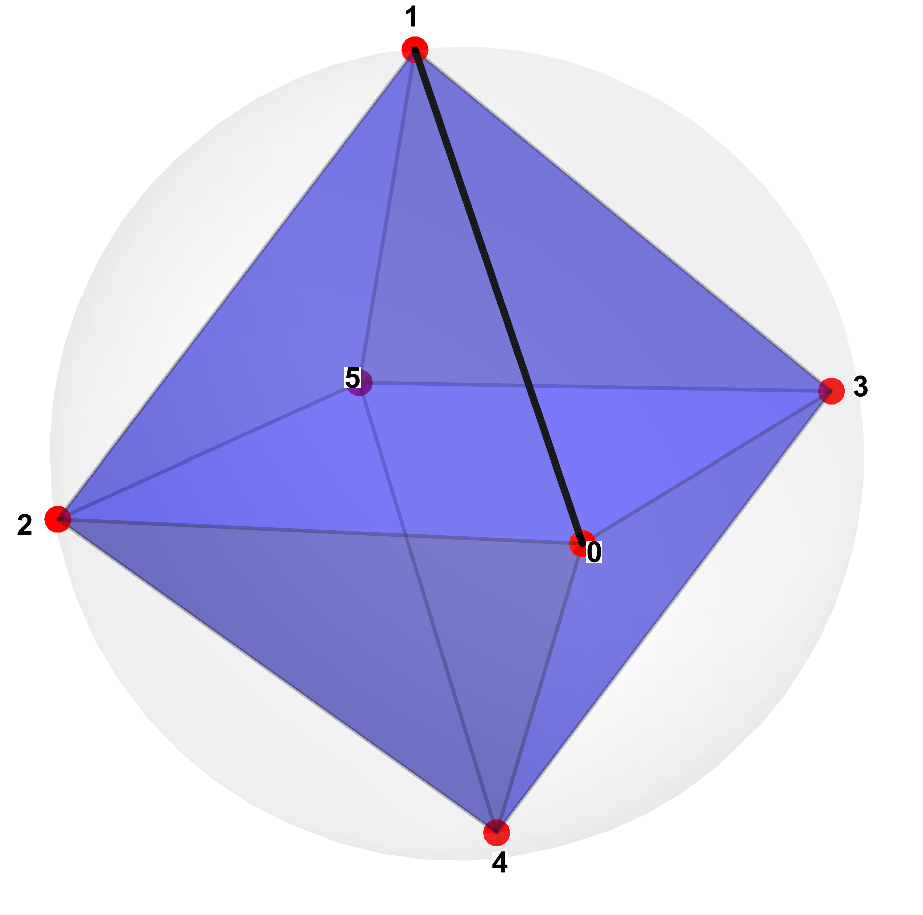
\includegraphics[width=.6\linewidth]{octahedron}
\end{center}

\begin{itemize}[leftmargin=1.5em]
  \item \textbf{Duality / paired solid:} cube
  \item \textbf{Vertices (V), Faces (F), Edges (E):} $V = 6$,\; $F = 8$ (equilateral triangles),\; $E = 12$
  \item \textbf{Point group:} $O_h$
  \item \textbf{Hilbert space:} \(
        \dim\mathcal{H} = 2^{6} = 64\ \text{(spin-$\tfrac12$ on each vertex)}
        \)
  \item \textbf{Eigenvalue range:} $[-18.80, 19.67]$
\end{itemize}

\subsubsection*{Scar structure: sets and multiplets}

\begin{itemize}[leftmargin=1.5em]
  \item \textbf{Number of scar sets:} 3
  \end{itemize}
  \hspace{6mm}For each scar set $S_k$:\\

\begin{center}
\begin{tabular}{L{3.5cm} C{2.2cm} C{2.2cm} C{2.2cm} C{3.0cm} C{3.2cm}}
\toprule
\textbf{Multiplet label} & \textbf{Energy $E$} & \textbf{Degeneracy} & \textbf{Annihilated by} & \textbf{Non-zero components (vs.\ $2^{6} = 64$)} \\
\midrule
$S_1$ & -6 & 3  & $\Hising$ & 12 \\
\midrule
$S_2$ & -4 & 1 & $\Htf$ & 12 \\
\midrule
$S_3$ & 6 & 3 & $\Hising$ & 12 \\
\bottomrule
\end{tabular}
\end{center}

\subsubsection*{Local properties (RDMs)}

\begin{itemize}[leftmargin=1.5em]
  \item \textbf{Local RDM definition:} $\rho_A=\mathrm{Tr}_{\bar A}(|\psi\rangle\langle\psi|)$ on compact subsets of $n=2$ sites, with $n < V/2, (V=6)$
  \item \textbf{Compactness criterion:} nearest-neighbor, for example $[0,1]$ (see highlighted edges in figure)
   \item \textbf{Diagnostics:} 2-sites RDMs for all 7 scars have full rank (system size $V=6$ is too small)
\end{itemize}

% -------------------- Polyhedron Block: END --------------------

% -------------------- Polyhedron Block: START --------------------
\subsection*{Cube}

\subsubsection*{Overview and data}
\begin{center}
  % Put your graphic at the very beginning of the subparagraph
  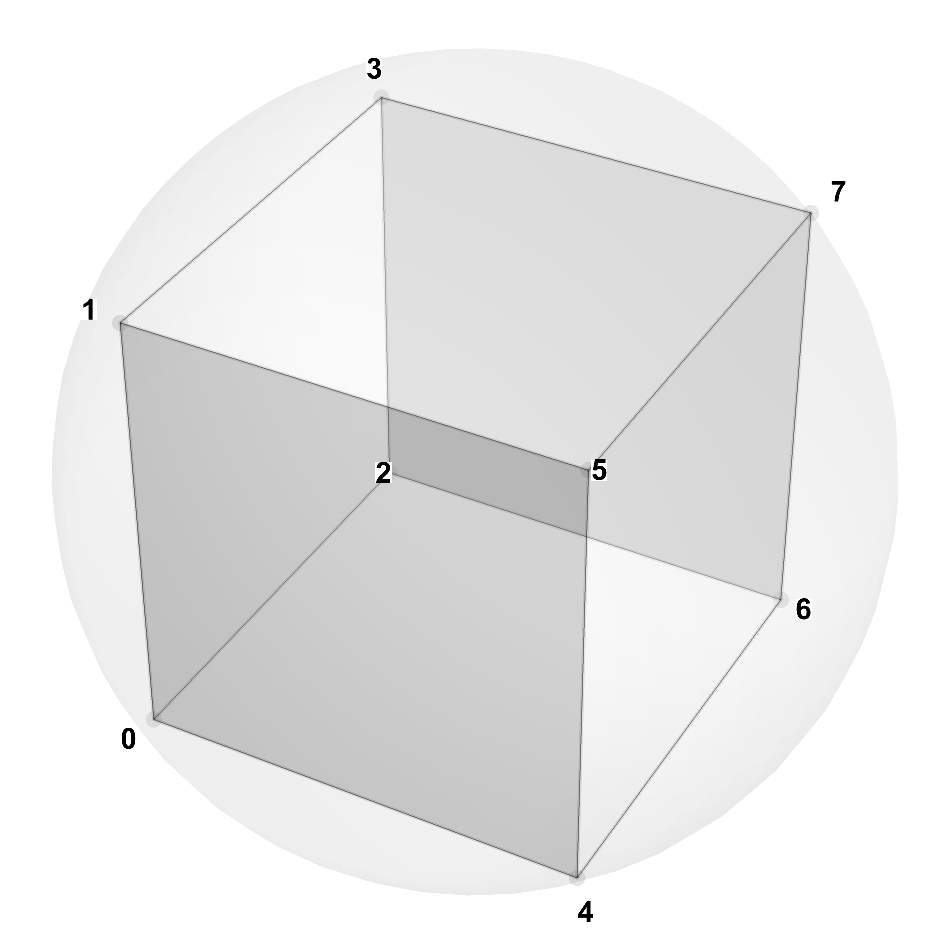
\includegraphics[width=.6\linewidth]{cube}
\end{center}

\begin{itemize}[leftmargin=1.5em]
  \item \textbf{Duality / paired solid:} octahedron
  \item \textbf{Vertices (V), Faces (F), Edges (E):} $V = 8$,\; $F = 6$ (squares),\; $E = 12$
  \item \textbf{Point group:} $O_h$
  \item \textbf{Hilbert space:} \(
        \dim\mathcal{H} = 2^{8} = 256\ \text{(spin-$\tfrac12$ on each vertex)}
        \)
  \item \textbf{Eigenvalue range:} $[-25.11, 25.11]$
\end{itemize}

\subsubsection*{Scar structure: sets and multiplets}

\begin{itemize}[leftmargin=1.5em]
  \item \textbf{Number of scar sets:} 2
  \end{itemize}
  \hspace{6mm}For each scar set $S_k$:\\

\begin{center}
\begin{tabular}{L{3.5cm} C{2.2cm} C{2.2cm} C{2.2cm} C{3.0cm} C{3.2cm}}
\toprule
\textbf{Multiplet label} & \textbf{Energy $E$} & \textbf{Degeneracy} & \textbf{Annihilated by} & \textbf{Non-zero components (vs.\ $2^{8} = 256$)} \\
\midrule
$S_1$ & -2 & 3 & $\Htf$ & 48 \\
\midrule
$S_2$ & 2 & 3 & $\Htf$ & 48 \\
\bottomrule
\end{tabular}
\end{center}

\subsubsection*{Local properties (RDMs)}

\begin{itemize}[leftmargin=1.5em]
  \item \textbf{Local RDM definition:} $\rho_A=\mathrm{Tr}_{\bar A}(|\psi\rangle\langle\psi|)$ on compact subsets of $n=2,3$ sites, with $n < V/2, (V = 8)$
  \item \textbf{Compactness criterion:} nearest-neighbor + most compact, for example $[0,1] (n = 2), [0,1,2] (n = 3)$ (see highlighted edges in figure)
  \item \textbf{Diagnostics:} 2/3-sites RDMs for all 6 scars have full rank (system size $V=8$ is too small)
\end{itemize}

% -------------------- Polyhedron Block: END --------------------

% -------------------- Polyhedron Block: START --------------------
\subsection*{Icosahedron}

\subsubsection*{Overview and data}

\begin{center}
  \begin{minipage}[c]{0.45\linewidth}
    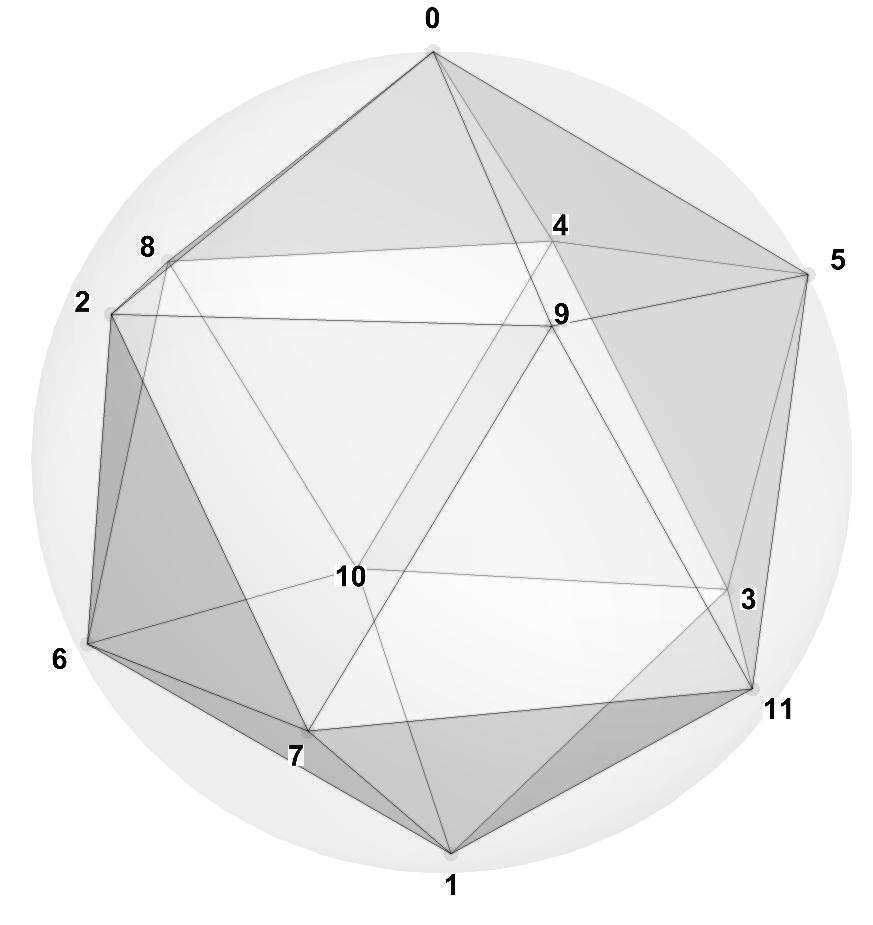
\includegraphics[width=\linewidth]{icosahedron}
  \end{minipage}\hfill
  \begin{minipage}[c]{0.45\linewidth}
    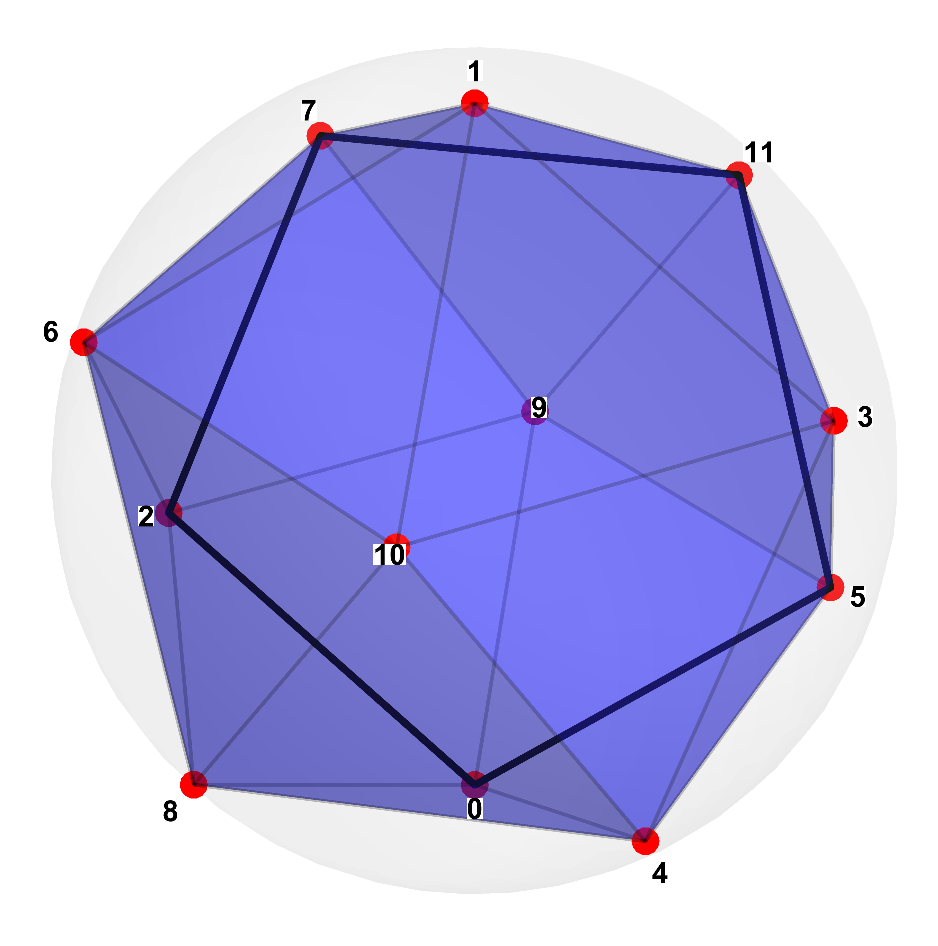
\includegraphics[width=\linewidth]{icosahedronp}
  \end{minipage}
\end{center}

\begin{itemize}[leftmargin=1.5em]
  \item \textbf{Duality / paired solid:} dodecahedron
  \item \textbf{Vertices (V), Faces (F), Edges (E):} $V = 12$,\; $F = 20$ (equilateral triangles),\; $E = 30$
  \item \textbf{Point group:} $I_h$
  \item \textbf{Hilbert space:} \(
        \dim\mathcal{H} = 2^{12} = 4096\ \text{(spin-$\tfrac12$ on each vertex)}
        \)
  \item \textbf{Eigenvalue range:} $[-37.95, 41.29]$
\end{itemize}

\subsubsection*{Scar structure: sets and multiplets}

\begin{itemize}[leftmargin=1.5em]
  \item \textbf{Number of scar sets:} 1
  \end{itemize}
  \hspace{6mm}For each scar set $S_k$:\\

\begin{center}
\begin{tabular}{L{3.5cm} C{2.2cm} C{2.2cm} C{2.2cm} C{3.0cm} C{3.2cm}}
\toprule
\textbf{Multiplet label} & \textbf{Energy $E$} & \textbf{Degeneracy} & \textbf{Annihilated by} & \textbf{Non-zero components (vs.\ $2^{12} = 4096$)} \\
\midrule
$S_1$ & -6 & 5 & $\Htf$ & 280 \\
\bottomrule
\end{tabular}
\end{center}
  
\noindent *We have also observed two additional, non-degenerate ``scarred'' states (let's call them ``pseudoscars'') at integer energies $E=0,-4$, which are less sparse than the five-fold scarred multiplet, but are still sparser than the other eigenstates. These two pseudoscars have the peculiarity that they are not annihilated by either $\Hising , \Htf$, and they are not even eigenstates of them (like it happens for the other scars), but instead their expectation value of  $\Htf$ is zero (for the pseudoscar at $E=0$, the expectation value of $\Hising$ is also zero). If $|s\rangle$ is the scarred eigenstate of $H$ corresponding to either $E=0,-4$, we have that:

\begin{equation}
\langle s|  H_{\text{TF}} |s \rangle = 0
\end{equation}

In other words,  $H_{\text{TF}}$ projects $|s\rangle$ onto its orthogonal complement, causing the expectation value to be zero.\\

\begin{center}
\begin{tabular}{L{3.5cm} C{2.2cm} C{2.2cm} C{2.2cm} C{3.0cm} C{3.2cm}}
\toprule
\textbf{Multiplet label} & \textbf{Energy $E$} & \textbf{Degeneracy} & \textbf{Annihilated by} & \textbf{Non-zero components (vs.\ $2^{12} = 4096$)} \\
\midrule
$S'_1$ & -4 & 1 & neither & 720 \\
$S'_2$ & 0 & 1 & neither & 600 \\
\bottomrule
\end{tabular}
\end{center}

There are additional sparser eigenvectors which are not integer:

\begin{itemize}
\item 480 non-zero components: E= -8.64, -5.85, 3.85, 6.64 
\item 840 non-zero components: E= -16.87, -12.87, -8.27, -4.27, 0.27, 4.27, 8.87, 12.87 
\end{itemize}

\subsubsection*{Local properties (RDMs)}

\begin{itemize}[leftmargin=1.5em]
  \item \textbf{Local RDM definition:} $\rho_A=\mathrm{Tr}_{\bar A}(|\psi\rangle\langle\psi|)$ on compact subsets of $n=2,3,4,5$ sites, with $n < V/2, (V=12)$.
  \item \textbf{Compactness criterion:} nearest-neighbor + most compact, for example $[0,2] \, (n = 2),$ \\ $[0,2,9] \, (n = 3), [0,2,7,9] \,  (n = 4), [0,2,7,9,11] \, (n = 5)$; for the pseudoscars, for n=5 we looked at the pentagon [0,2,5,7,11] (see highlighted edges in figure; first n=5 [0,2,7,9,11] is highlighted in the figure on the left, while n=5 [0,2,5,7,11] is highlighted in the figure on the right).
  \item \textbf{Diagnostics:} \begin{itemize} \item 2/3-sites RDMs for all 5 scars + 2 pseudoscars have full rank \item 4-sites RDMs for all 5 scars have reduced rank of 11 = 16 - 5; 2 pseudoscars have full rank \item 5-sites ([0,2,7,9,11]) RDMs for all 5 scars have reduced rank of 18 = 32 - 14, while the 2 pseudoscars have full rank; for the pentagon 5-sites [0,2,5,7,11], the 2 pseudoscars (together with the other non-integer sparser eigenvectors found above) have both reduced rank of 32 - 8 = 24 (the 5 scars have also reduced rank of 32 - 6 = 26)\end{itemize}
\end{itemize}

\subsubsection*{Observation on pseudoscars}

The two pseudoscars at integer energies $E=0,-4$ do not have sub-volume entanglement entropy (like for the scars studied in literature so far), but still show reduced rank for appropriately chosen local RDMs, such as the 5-sites pentagon one. This suggests that the two pseudoscars - if they are of any interest - are better characterized in terms of the FRH (Full Rank Hypothesis) rather than the ETH (Eigenstate Thermalization Hypothesis).

% -------------------- Polyhedron Block: END --------------------

% -------------------- Polyhedron Block: START --------------------
\subsection*{Dodecahedron}

\subsubsection*{Overview and data}
\begin{center}
  % Put your graphic at the very beginning of the subparagraph
  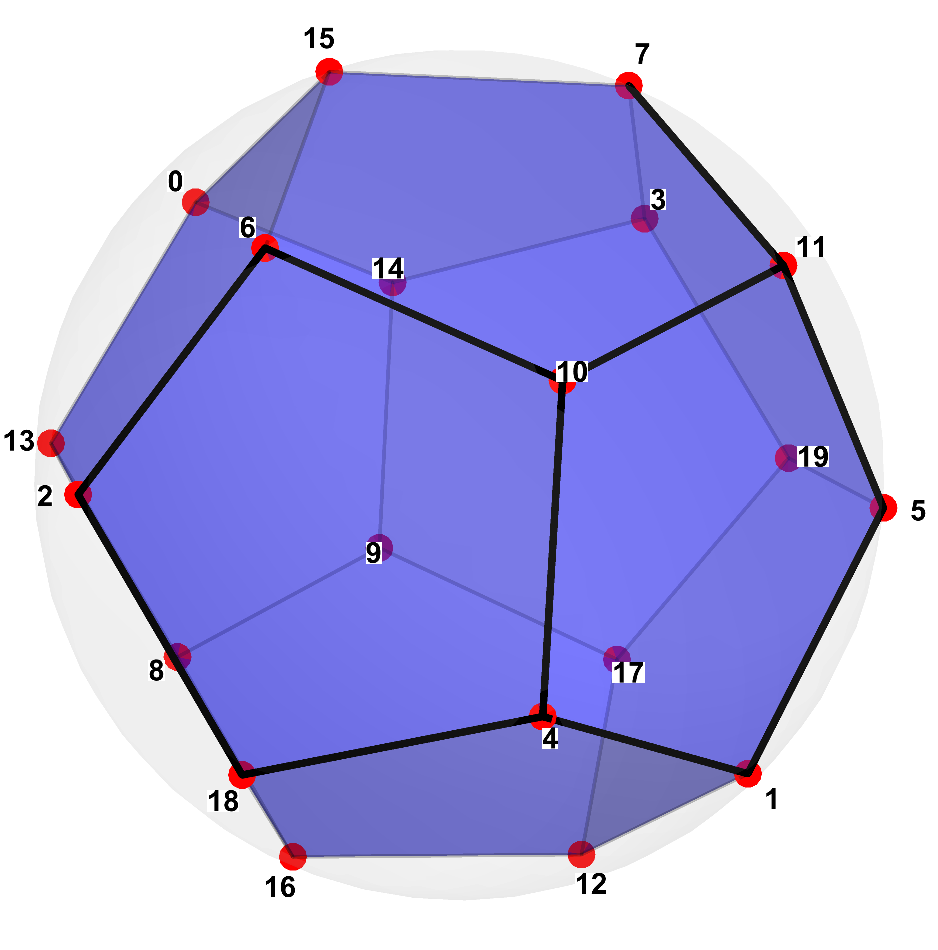
\includegraphics[width=.6\linewidth]{dodecahedron}
\end{center}

\begin{itemize}[leftmargin=1.5em]
  \item \textbf{Duality / paired solid:} icosahedron
  \item \textbf{Vertices (V), Faces (F), Edges (E):} $V = 20$,\; $F = 12$ (pentagons),\; $E = 30$
  \item \textbf{Point group:} $I_h$
  \item \textbf{Hilbert space:} \(
        \dim\mathcal{H} = 2^{20} = 1,048,576\ \text{(spin-$\tfrac12$ on each vertex)}
        \)
  \item \textbf{Eigenvalue range:} $[-62.51, 62.61]$
\end{itemize}

\subsubsection*{Scar structure: sets and multiplets}

\begin{itemize}[leftmargin=1.5em]
  \item \textbf{Number of scar sets:} 1
  \end{itemize}
  \hspace{6mm}For each scar set $S_k$:\\

\begin{center}
\begin{tabular}{L{3.5cm} C{2.2cm} C{2.2cm} C{2.2cm} C{3.0cm} C{3.2cm}}
\toprule
\textbf{Multiplet label} & \textbf{Energy $E$} & \textbf{Degeneracy} & \textbf{Annihilated by} & \textbf{Non-zero components (vs.\ $2^{20} = 1,048,576$)} \\
\midrule
$S_1$ &  & & $\Htf$ & \\
\bottomrule
\end{tabular}
\end{center}

\subsubsection*{Local properties (RDMs)}

\begin{itemize}[leftmargin=1.5em]
  \item \textbf{Local RDM definition:} $\rho_A=\mathrm{Tr}_{\bar A}(|\psi\rangle\langle\psi|)$ on compact subsets of $n=2,3,4,5,6,7,8,9$ sites, with $n < V/2, (V=20)$
  \item \textbf{Compactness criterion:} nearest-neighbor + most compact, for example $[4,10] \, (n = 2), [4,6,10] \, (n = 3), [2,4,6,10] \,  (n = 4), [2,4,6,10,18] \, (n = 5), [1,2,4,6,10,18] \, (n = 6), \newline
   [1,2,4,5,6,10,18] \, (n = 7), [1,2,4,5,6,10,11,18] \, (n = 8), [1,2,4,5,6,7,10,11,18] \, (n = 9)$ (see highlighted edges in figure)
  \item \textbf{Diagnostics:} \begin{itemize} \item 2/3-sites RDMs for all scars have full rank \item 4-sites RDMs for all scars have reduced rank \item 5-sites RDMs for all scars have reduced rank\item 6-sites RDMs for all scars have reduced rank
  \item 7-sites RDMs for all scars have reduced rank \item 8-sites RDMs for all scars have reduced rank \item 9-sites RDMs for all scars have reduced rank\end{itemize}
\end{itemize}

% -------------------- Polyhedron Block: END --------------------

\section*{Catalan Solids}
% ============================================================
% REPEAT THE BLOCK BELOW FOR EACH POLYHEDRON
% ============================================================

% -------------------- Polyhedron Block: START --------------------
\subsection*{Triakis Tetrahedron}

\subsubsection*{Overview and data}
\begin{center}
  % Put your graphic at the very beginning of the subparagraph
  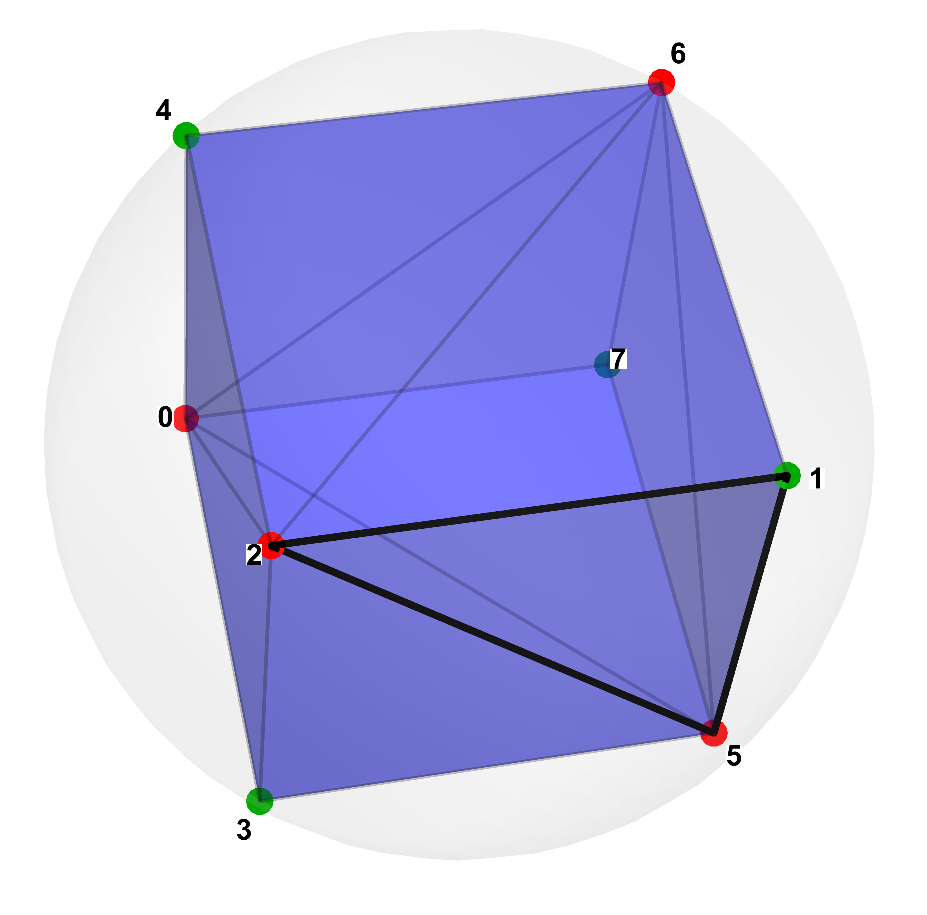
\includegraphics[width=.6\linewidth]{triakistetrahedron}
\end{center}

\begin{itemize}[leftmargin=1.5em]
  \item \textbf{Duality / paired solid:} truncated tetrahedron (archimedean)
  \item \textbf{Vertices (V), Faces (F), Edges (E):} $V = 8$ (4 on the primary tetrahedron, 4 at the tip of the 4 pyramids built on top of each face of the tetrahedron),\; $F = 12$ (isosceles triangles),\; $E = 18$
  \item \textbf{Point group:} $T_d$
  \item \textbf{Hilbert space:} \(
        \dim\mathcal{H} = 2^{8} = 256\ \text{(spin-$\tfrac12$ on each vertex)}
        \)
  \item \textbf{Eigenvalue range:} $[-25.10, 27.07]$
\end{itemize}

\subsubsection*{Scar structure: sets and multiplets}

\begin{itemize}[leftmargin=1.5em]
  \item \textbf{Number of scar sets:} 1
  \end{itemize}
  \hspace{6mm}For each scar set $S_k$:\\

\begin{center}
\begin{tabular}{L{3.5cm} C{2.2cm} C{2.2cm} C{2.2cm} C{3.0cm} C{3.2cm}}
\toprule
\textbf{Multiplet label} & \textbf{Energy $E$} & \textbf{Degeneracy} & \textbf{Annihilated by} & \textbf{Non-zero components (vs.\ $2^{8} = 256$)} \\
\midrule
$S_1$ & -2 & 3 & $\Htf$ & 36\\
\bottomrule
\end{tabular}
\end{center}

\subsubsection*{Local properties (RDMs)}

\begin{itemize}[leftmargin=1.5em]
  \item \textbf{Local RDM definition:} $\rho_A=\mathrm{Tr}_{\bar A}(|\psi\rangle\langle\psi|)$ on compact subsets of $n=2,3$ sites, with $n < V/2, (V=8)$
  \item \textbf{Compactness criterion:} nearest-neighbor + most compact, for example $[1,2] (n = 2), [1,2,5] (n = 3)$ (see highlighted edges in figure)
  \item \textbf{Diagnostics:} 2/3-sites RDMs for all 3 scars have full rank (system size $V=8$ is too small)
\end{itemize}

% -------------------- Polyhedron Block: END ---------------------

% -------------------- Polyhedron Block: START --------------------
\subsection*{Rhombic Dodecahedron}

\subsubsection*{Overview and data}
\begin{center}
  % Put your graphic at the very beginning of the subparagraph
  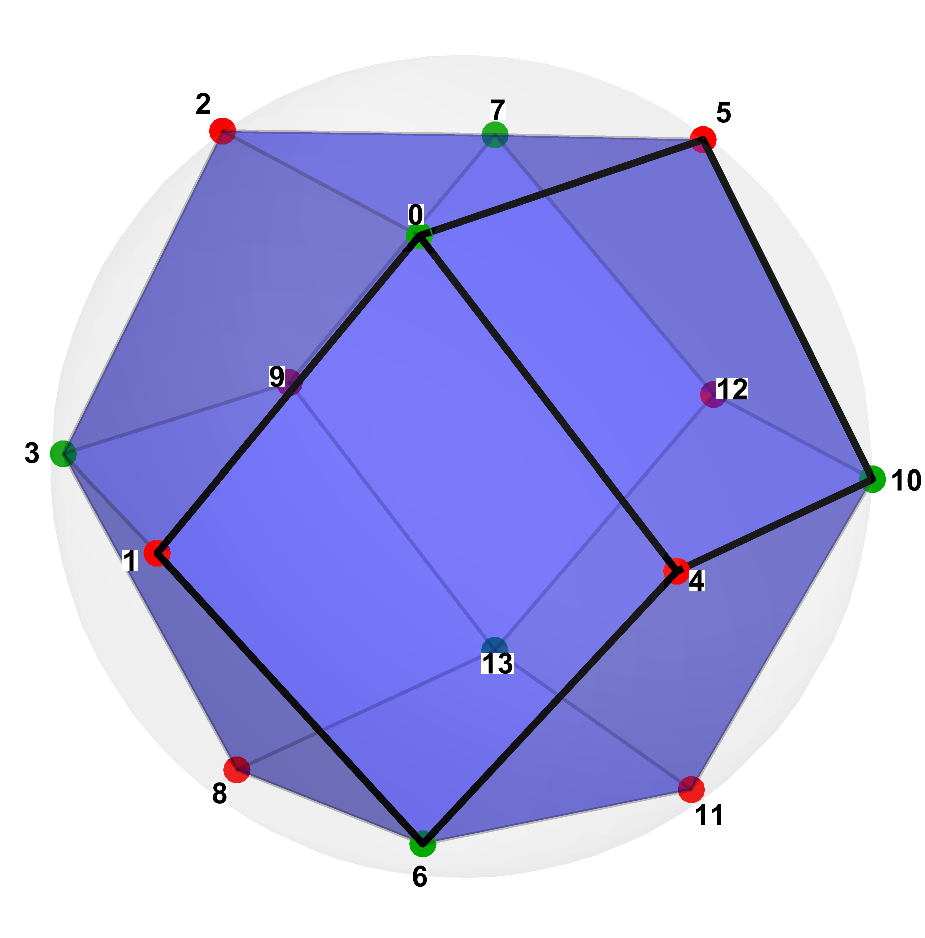
\includegraphics[width=.6\linewidth]{rhombicdodecahedron}
\end{center}

\begin{itemize}[leftmargin=1.5em]
  \item \textbf{Duality / paired solid:} cuboctahedron (archimedean)
  \item \textbf{Vertices (V), Faces (F), Edges (E):} $V = 14$ (8 acute vertices where 3 rhombi meet, 6 obtuse vertices where 4 rhombi meet),\; $F = 12$ (rhombi),\; $E = 24$
  \item \textbf{Point group:} $O_h$
  \item \textbf{Hilbert space:} \(
        \dim\mathcal{H} = 2^{14} = 16,384\ \text{(spin-$\tfrac12$ on each vertex)}
        \)
  \item \textbf{Eigenvalue range:} $[-44.28, 44.28]$
\end{itemize}

\subsubsection*{Scar structure: sets and multiplets}

\begin{itemize}[leftmargin=1.5em]
  \item \textbf{Number of scar sets:} 4
  \end{itemize}
  \hspace{6mm}For each scar set $S_k$:\\

\begin{center}
\begin{tabular}{L{3.5cm} C{2.2cm} C{2.2cm} C{2.2cm} C{3.0cm} C{3.2cm}}
\toprule
\textbf{Multiplet label} & \textbf{Energy $E$} & \textbf{Degeneracy} & \textbf{Annihilated by} & \textbf{Non-zero components (vs.\ $2^{14} = 16,384$)} \\
\midrule
$S_1$ & -12 & 3 & $\Hising$ & 432\\
\midrule
$S_2$ & -6 & 18 & $\Hising$ & 432\\
\midrule
$S_3$ & 6 & 18 & $\Hising$ & 432\\
\midrule
$S_4$ & 12 & 3 & $\Hising$ & 432\\
\bottomrule
\end{tabular}
\end{center}

\subsubsection*{Local properties (RDMs)}

\begin{itemize}[leftmargin=1.5em]
  \item \textbf{Local RDM definition:} $\rho_A=\mathrm{Tr}_{\bar A}(|\psi\rangle\langle\psi|)$ on compact subsets of $n=2,3,4,5,6$ sites, with $n < V/2, (V=14)$
  \item \textbf{Compactness criterion:} nearest-neighbor + most compact, for example $[0,1] \, (n = 2), [0,1,4] \, (n = 3), [0,1,4,6] \,  (n = 4), [0,1,5,6,10] \, (n = 5), [0,1,4,5,6,10] \, (n = 6)$ (see highlighted edges in figure)
  \item \textbf{Diagnostics:} \begin{itemize} \item 2/3-sites RDMs for all scars have full rank \item 4-sites RDMs for the $S_1,S_4$ scars have reduced rank of 12, and for $S_2,S_3$ have full rank \item 5-sites RDMs for the $S_1,S_4$ scars have reduced rank of 16, and for $S_2,S_3$ have reduced rank of 28 \item 6-sites RDMs for the $S_1,S_4$ scars have reduced rank of 20, and for $S_2,S_3$ have reduced rank of 50 \end{itemize}
\end{itemize}

% -------------------- Polyhedron Block: END --------------------

% -------------------- Polyhedron Block: START --------------------
\subsection*{Triakis Octahedron}

\subsubsection*{Overview and data}
\begin{center}
  % Put your graphic at the very beginning of the subparagraph
  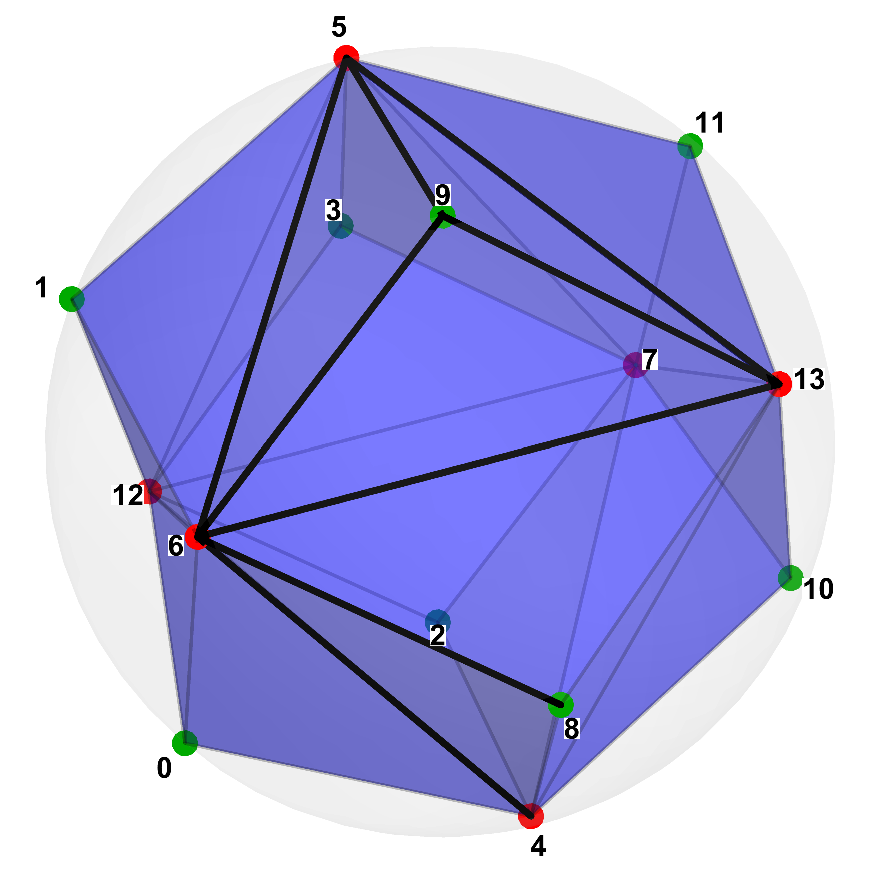
\includegraphics[width=.6\linewidth]{triakisoctahedron}
\end{center}

\begin{itemize}[leftmargin=1.5em]
  \item \textbf{Duality / paired solid:} truncated cube (archimedean)
  \item \textbf{Vertices (V), Faces (F), Edges (E):} $V = 14$ (6 on the primary octahedron, 8 at the tip of the 8 pyramids built on top of each face of the octahedron),\; $F = 24$ (isosceles triangles),\; $E = 36$
  \item \textbf{Point group:} $O_h$
  \item \textbf{Hilbert space:} \(
        \dim\mathcal{H} = 2^{14} = 16,384\ \text{(spin-$\tfrac12$ on each vertex)}
        \)
  \item \textbf{Eigenvalue range:} $[-44.21, 50.01]$
\end{itemize}

\subsubsection*{Scar structure: sets and multiplets}

\begin{itemize}[leftmargin=1.5em]
  \item \textbf{Number of scar sets:} 2
  \end{itemize}
  \hspace{6mm}For each scar set $S_k$:\\

\begin{center}
\begin{tabular}{L{3.5cm} C{2.2cm} C{2.2cm} C{2.2cm} C{3.0cm} C{3.2cm}}
\toprule
\textbf{Multiplet label} & \textbf{Energy $E$} & \textbf{Degeneracy} & \textbf{Annihilated by} & \textbf{Non-zero components (vs.\ $2^{14} = 16,384$)} \\
\midrule
$S_1$ & -4 & 1 & $\Htf$ & 192 \\
\midrule
$S_2$ & 0 & 4 & both\footnotemark & 368 \\
\bottomrule
\end{tabular}
\end{center}

\footnotetext{The eigenvalues are not exactly zero for $\Hising$, but very small, of the order of $10^{-13/14}$.}

\subsubsection*{Local properties (RDMs)}

\begin{itemize}[leftmargin=1.5em]
  \item \textbf{Local RDM definition:} $\rho_A=\mathrm{Tr}_{\bar A}(|\psi\rangle\langle\psi|)$ on compact subsets of $n=2,3,4,5,6$ sites, with $n < V/2, (V=14)$
  \item \textbf{Compactness criterion:} nearest-neighbor + most compact, for example $[5,6] \, (n = 2), [5,6,9] \, (n = 3), [5,6,9,13] \,  (n = 4), [4,5,6,9,13] \, (n = 5), [4,5,6,8,9,13] \, (n = 6)$ (see highlighted edges in figure)
  \item \textbf{Diagnostics:} \begin{itemize} \item 2/3-sites RDMs for all scars have full rank \item 4-sites RDMs for the $S_1$ scar have reduced rank of 8, and for $S_2$ have full rank \item 5-sites RDMs for the $S_1$ scar have reduced rank of 8, and for $S_2$ have reduced rank of 16 \item 6-sites RDMs for the $S_1$ scar have reduced rank of 16, and for $S_2$ have reduced rank of 20 \end{itemize}
\end{itemize}

% -------------------- Polyhedron Block: END --------------------

% -------------------- Polyhedron Block: START --------------------
\subsection*{Tetrakis Hexahedron}

\subsubsection*{Overview and data}
\begin{center}
  % Put your graphic at the very beginning of the subparagraph
  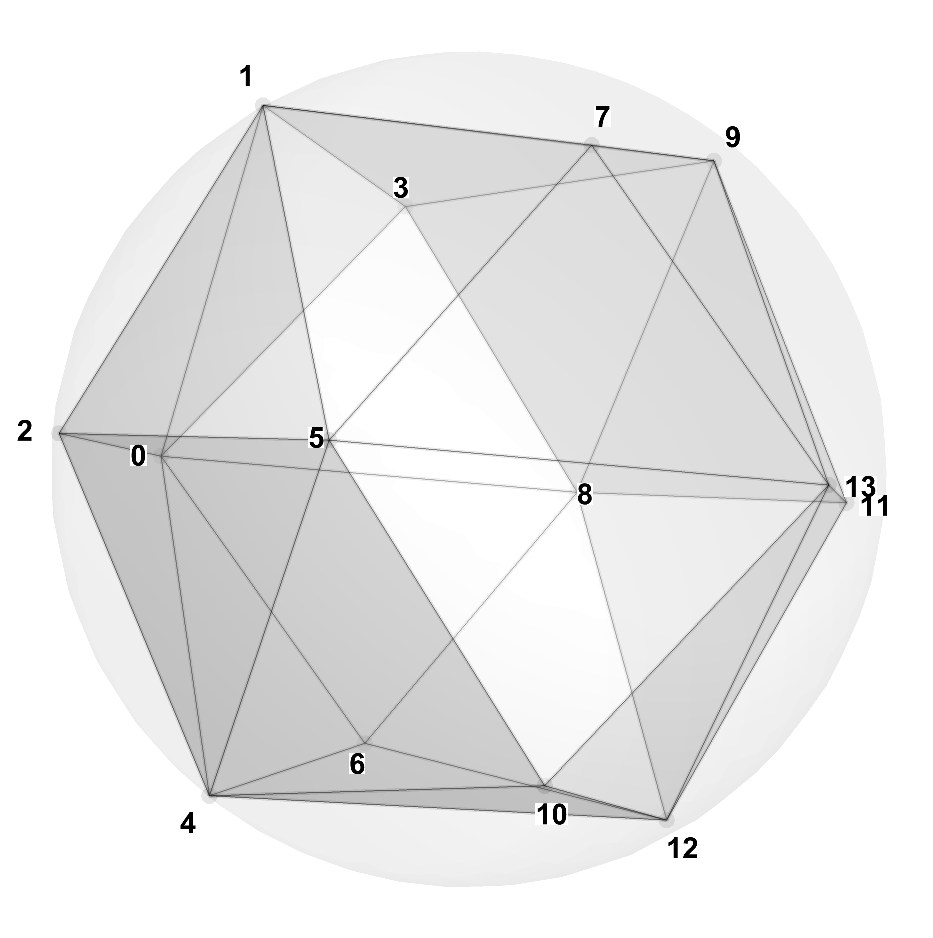
\includegraphics[width=.6\linewidth]{tetrakishexahedron}
\end{center}

\begin{itemize}[leftmargin=1.5em]
  \item \textbf{Duality / paired solid:} truncated octahedron (archimedean)
  \item \textbf{Vertices (V), Faces (F), Edges (E):} $V = 14$  (8 on the primary cube/hexahedron, 6 at the tip of the 8 pyramids built on top of each face of the cube/hexahedron),\; $F = 24$ (isosceles triangles),\; $F = 24$ (isosceles triangles),\; $E = 36$
  \item \textbf{Point group:} $O_h$
  \item \textbf{Hilbert space:} \(
        \dim\mathcal{H} = 2^{14} = 16,384\ \text{(spin-$\tfrac12$ on each vertex)}
        \)
  \item \textbf{Eigenvalue range:} $[-44.39, 48.90]$
\end{itemize}

\subsubsection*{Scar structure: sets and multiplets}

\begin{itemize}[leftmargin=1.5em]
  \item \textbf{Number of scar sets:} 2
  \end{itemize}
  \hspace{6mm}For each scar set $S_k$:\\

\begin{center}
\begin{tabular}{L{3.5cm} C{2.2cm} C{2.2cm} C{2.2cm} C{3.0cm} C{3.2cm}}
\toprule
\textbf{Multiplet label} & \textbf{Energy $E$} & \textbf{Degeneracy} & \textbf{Annihilated by} & \textbf{Non-zero components (vs.\ $2^{14} = 16,384$)} \\
\midrule
$S_1$ & -4 & 12 & $\Htf$ & 1172 \\
\midrule
$S_2$ & 0 & 1 & both\footnotemark & 192 \\
\bottomrule
\end{tabular}
\end{center}

\footnotetext{The eigenvalue is not exactly zero for $\Hising$, but very small, of the order of $10^{-14}$.}

\subsubsection*{Local properties (RDMs)}

\begin{itemize}[leftmargin=1.5em]
  \item \textbf{Local RDM definition:} $\rho_A=\mathrm{Tr}_{\bar A}(|\psi\rangle\langle\psi|)$ on compact subsets of $n=2,3,4,5,6$ sites, with $n < V/2, (V=14)$
  \item \textbf{Compactness criterion:} nearest-neighbor + most compact, for example $[1,5] \, (n = 2), [1,5,7] \, (n = 3), [1,5,9,13] \,  (n = 4), [1,5,7,9,13] \, (n = 5), [0,1,5,7,9,13] \, (n = 6)$ (see highlighted edges in figure)
  \item \textbf{Diagnostics:} \begin{itemize} \item 2/3-sites RDMs for all scars have full rank \item 4-sites RDMs for the $S_1$ scars have full rank, and for $S_2$ have reduced rank of 6  \item 5-sites RDMs for the $S_1$ scar have reduced rank of 26, and for $S_2$ have reduced rank of 12 \item 6-sites RDMs for the $S_1$ scar have reduced rank of 52, and for $S_2$ have reduced rank of 24 \end{itemize}
\end{itemize}


% -------------------- Polyhedron Block: END --------------------

\noindent\textbf{NB: in the triakis octahedron and tetrakis hexahedron there is a clear hierarchy of the vertices - the (red) vertices of the primary solids, the octahedron and the cube, are prioritized over the (green) vertices at the tip of the pyramids when computing reduced sites RDMs. This explains why the 6th vertices of 4 (for the triakis octahedron) and of 0 (for the tetrakis hexahedron) were respectively added to the 6-sites subset. Also, the vertices hierarchy forces to pick 4 primary vertices + 3 pyramid vertices when computing the bipartite entanglement entropy.}

\section*{Archimedean Solids}

\noindent\textbf{In this case, the hyerarchy is for the faces only. I am not even sure if this is a real hyerarchy - i.e. there are two types of faces, but is one type of face more important than the other? In the case of the truncated tetrahedron, which is the only archimedean solid studied with a scar, the bipartite entanglement entropy seems to be lower when prioritizing the traingular faces over the hexagonal ones. However, when computing 3/4/5-sites RDMs, none of the vertices combination, including the ones prioritizing the vertices on the triangular faces, seems to give a reduced rank RDM.}

% ============================================================
% REPEAT THE BLOCK BELOW FOR EACH POLYHEDRON
% ============================================================

% -------------------- Polyhedron Block: START --------------------
\subsection*{Truncated Tetrahedron}

\subsubsection*{Overview and data}
\begin{center}
  % Put your graphic at the very beginning of the subparagraph
  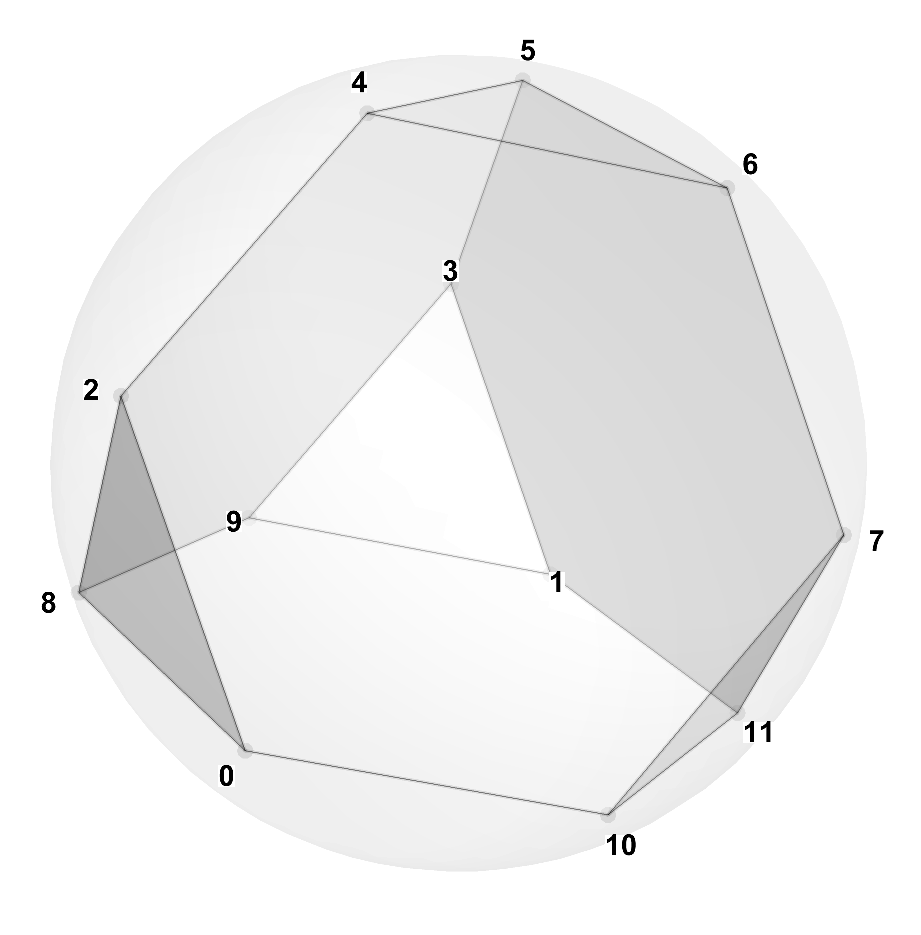
\includegraphics[width=.6\linewidth]{truncatedtetrahedron}
\end{center}

\begin{itemize}[leftmargin=1.5em]
  \item \textbf{Duality / paired solid:} triakis tetrahedron (catalan)
  \item \textbf{Vertices (V), Faces (F), Edges (E):} $V = 12$,\; $F = 8$ (4 equilateral triangles, 4 hexagons),\; $E = 18$
  \item \textbf{Point group:} $T_d$
  \item \textbf{Hilbert space:} \(
        \dim\mathcal{H} = 2^{12} = 4,096\ \text{(spin-$\tfrac12$ on each vertex)}
        \)
  \item \textbf{Eigenvalue range:} $[-37.36, 37.71]$
\end{itemize}

\subsubsection*{Scar structure: sets and multiplets}

\begin{itemize}[leftmargin=1.5em]
  \item \textbf{Number of scar sets:} 1
  \end{itemize}
  \hspace{6mm}For each scar set $S_k$:\\

\begin{center}
\begin{tabular}{L{3.5cm} C{2.2cm} C{2.2cm} C{2.2cm} C{3.0cm} C{3.2cm}}
\toprule
\textbf{Multiplet label} & \textbf{Energy $E$} & \textbf{Degeneracy} & \textbf{Annihilated by} & \textbf{Non-zero components (vs.\ $2^{12} = 4,096$)} \\
\midrule
$S_1$ & 0 & 1 & both\footnotemark & 48\\
\bottomrule
\end{tabular}
\end{center}

\footnotetext{The eigenvalue is not exactly zero for $\Hising$, but very small, of the order of $10^{-14}$.}

\subsubsection*{Local properties (RDMs)}

\begin{itemize}[leftmargin=1.5em]
  \item \textbf{Local RDM definition:} $\rho_A=\mathrm{Tr}_{\bar A}(|\psi\rangle\langle\psi|)$ on compact subsets of $n=2,3,4,5$ sites, with $n < V/2, (V=12)$
  \item \textbf{Compactness criterion:} nearest-neighbor + most compact, for example $[0,2] \, (n = 2), [0,2,8] \, (n = 3), [2,3,4,5] \,  (n = 4), [2,3,4,5,9] \, (n = 5)$ (see highlighted edges in figure)
  \item \textbf{Diagnostics:} all RDMs for the scar have full rank
\end{itemize}

% -------------------- Polyhedron Block: END --------------------

% -------------------- Polyhedron Block: START --------------------
\subsection*{Cuboctahedron}

\subsubsection*{Overview and data}
\begin{center}
  % Put your graphic at the very beginning of the subparagraph
  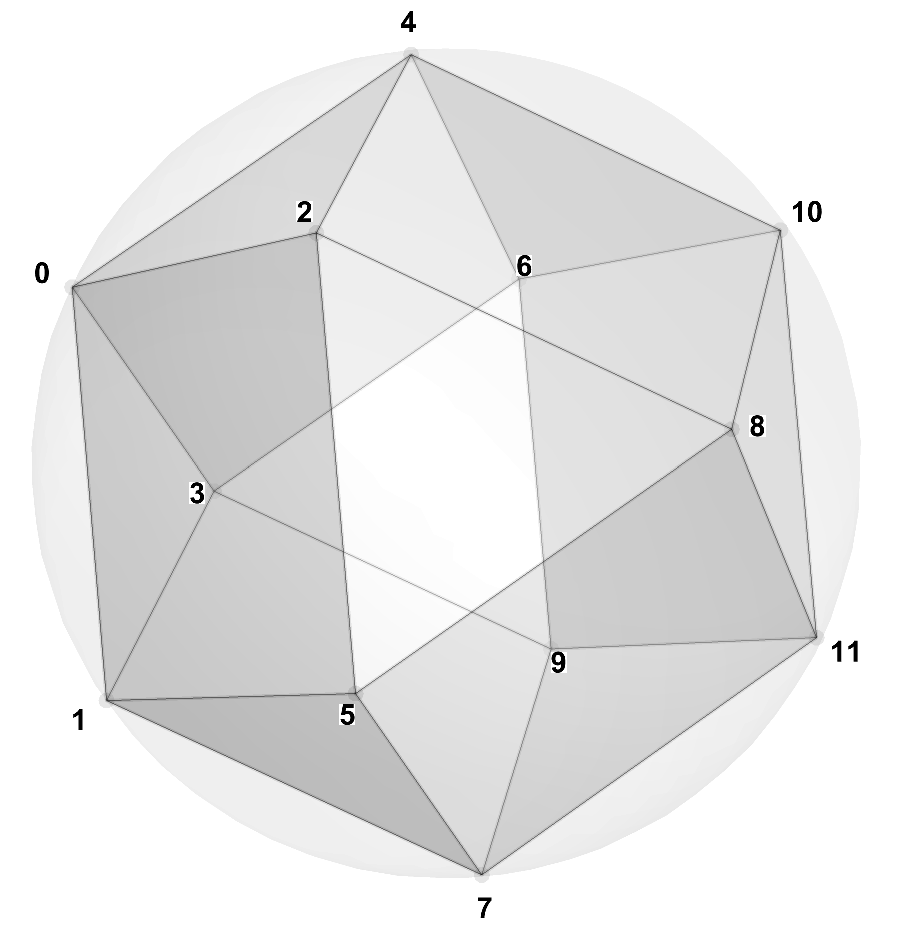
\includegraphics[width=.6\linewidth]{cuboctahedron}
\end{center}

\begin{itemize}[leftmargin=1.5em]
  \item \textbf{Duality / paired solid:} rhombic dodecahedron (catalan)
  \item \textbf{Vertices (V), Faces (F), Edges (E):} $V = 12$,\; $F = 14$ (8 equilateral triangles, 6 squares),\; $E = 24$
  \item \textbf{Point group:} $O_h$
  \item \textbf{Hilbert space:} \(
        \dim\mathcal{H} = 2^{12} = 4,096\ \text{(spin-$\tfrac12$ on each vertex)}
        \)
  \item \textbf{Eigenvalue range:} $[-37.73, 38.81]$
\end{itemize}

\subsubsection*{Scar structure: sets and multiplets}

\begin{itemize}[leftmargin=1.5em]
  \item \textbf{Number of scar sets:} no scars observed
  \end{itemize}

\subsubsection*{Local properties (RDMs)}

\begin{itemize}[leftmargin=1.5em]
  \item \textbf{Local RDM definition:} $\rho_A=\mathrm{Tr}_{\bar A}(|\psi\rangle\langle\psi|)$ on compact subsets of $n=2,3,4,5$ sites, with $n < V/2, (V=12)$
  \item \textbf{Compactness criterion:} nearest-neighbor + most compact, for example $[0,2] \, (n = 2), [0,2,4] \, (n = 3), [0,1,2,5] \,  (n = 4), [0,1,2,4,5] \, (n = 5)$ (see highlighted edges in figure)
  \item \textbf{Diagnostics:} all RDMs have full rank because there are no scars
\end{itemize}

% -------------------- Polyhedron Block: END --------------------

\paragraph*{Observations/Conclusions}

\begin{itemize}
\item The number of scars depends on whether the solid is Platonic, Catalan or Archimedean, and possibly it corresponds to the vertex orbits number of each solid class: Platonic and Archimedean solids have only 1 vertex orbit, since they are vertex-transitive, and so they have only 1 type of scar - up to algebraic sign (exception that I still do not understand: cuboctahedron doesn't seem to have any scar); Catalan solids have 2 vertex orbits, because they have two types of vertices, and they have two sets of scars, again up to an algebraic sign.\\
\item The degeneracy of each scarred multiplet depends on the point group $T_d, O_h, I_h$: For Platonic solids, the degeneracies are always 2 for $T_d$, 3 for $O_h$, and 5 for $I_h$. I am still not sure where these numbers come from, but my guess would be that they are related to the `'rotational'' symmetry subgroup of each point group. For Catalan and Archimedean solids, the description seems to be more complicated, because we have 2 types of vertices and faces, respectively, but it should follow a similar, more convoluted reasoning.
\item In some cases, the scarred multiplets come in symmetric pairs at $\pm n$, where $n\in\mathbb{N}$. I would like to think this is related to frustration - this seems to happen when the faces of each solid have an even number of vertices, and in this case the scars are usually annihilated by $\Hising$ and not by $\Htf$. There are however exception to this observation: in primis the octahedron, which shouldn't have symmetric scars since it has triangular faces, but it does; the cube, which despite having square faces, it does have a pair of symmetric scars, but these are annihilated by $\Htf$ and not  $\Hising$. This aspect is also confusing for Archimedean solids, since they have both even and odd-number of vertices faces.
\end{itemize}


\end{document}
